\documentclass{article}
\usepackage{tikz}
\usetikzlibrary{arrows.meta, positioning, shapes.geometric, fit, backgrounds}
\begin{document}

{\color{blue}
\begin{figure}[htbp]
    \centering
    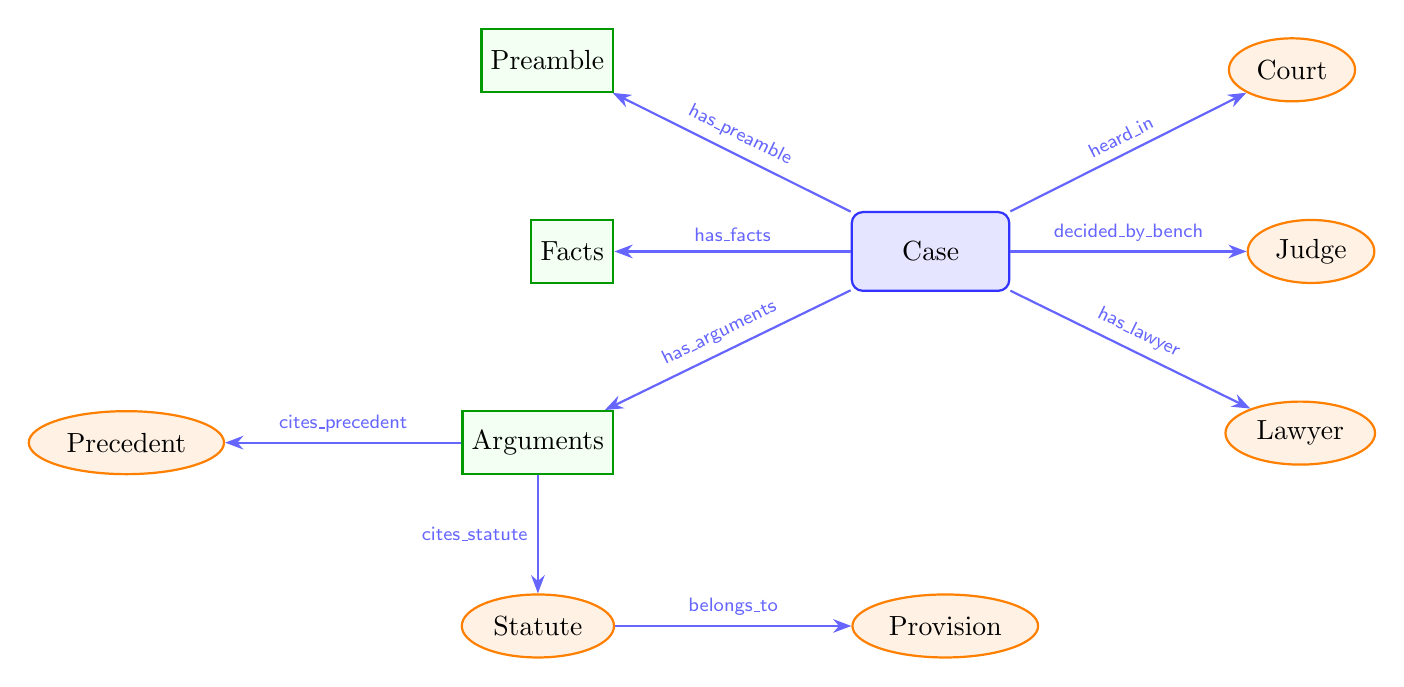
\begin{tikzpicture}[
        node distance=1.5cm and 3cm,
        case/.style={rectangle, rounded corners, draw=blue!80, fill=blue!10, thick, minimum width=2cm, minimum height=1cm, align=center},
        textnode/.style={rectangle, draw=green!60!black, fill=green!5, thick, minimum height=0.8cm, align=center},
        entity/.style={ellipse, draw=orange, fill=orange!10, thick, minimum height=0.8cm, align=center},
        edge/.style={->, >=Stealth, thick, blue!60, font=\scriptsize\sffamily, align=center}
    ]
        % Single case diagram
        \node[case] (case) {Case};
        
        \node[textnode, above left=of case] (preamble) {Preamble};
        \node[textnode, left=of case] (facts) {Facts};
        \node[textnode, below left=of case] (args) {Arguments};
        
        \node[entity, above right=of case] (court) {Court};
        \node[entity, right=of case] (judge) {Judge};
        \node[entity, below right=of case] (lawyer) {Lawyer};
        
        \node[entity, below=of args] (statute) {Statute};
        \node[entity, right=of statute] (provision) {Provision};
        
        \node[entity, left=of args] (precedent) {Precedent};

        \draw[edge] (case) -- node[above, sloped] {has\_preamble} (preamble);
        \draw[edge] (case) -- node[above, sloped] {has\_facts} (facts);
        \draw[edge] (case) -- node[above, sloped] {has\_arguments} (args);
        
        \draw[edge] (case) -- node[above, sloped] {heard\_in} (court);
        \draw[edge] (case) -- node[above, sloped] {decided\_by\_bench} (judge);
        \draw[edge] (case) -- node[above, sloped] {has\_lawyer} (lawyer);
        
        \draw[edge] (args) -- node[left] {cites\_statute} (statute);
        \draw[edge] (args) -- node[above] {cites\_precedent} (precedent);
        \draw[edge] (statute) -- node[above] {belongs\_to} (provision);

    \end{tikzpicture}
    \caption{\textcolor{blue}{Sample star-graph structure for a single Case node. Various text blocks feature as text nodes (left), while details like Court and Judge form entity nodes (right). The Arguments node branches out to cite Statutes and Precedents.}}
    \label{fig:single_case_graph}
\end{figure}

\begin{figure}[htbp]
    \centering
    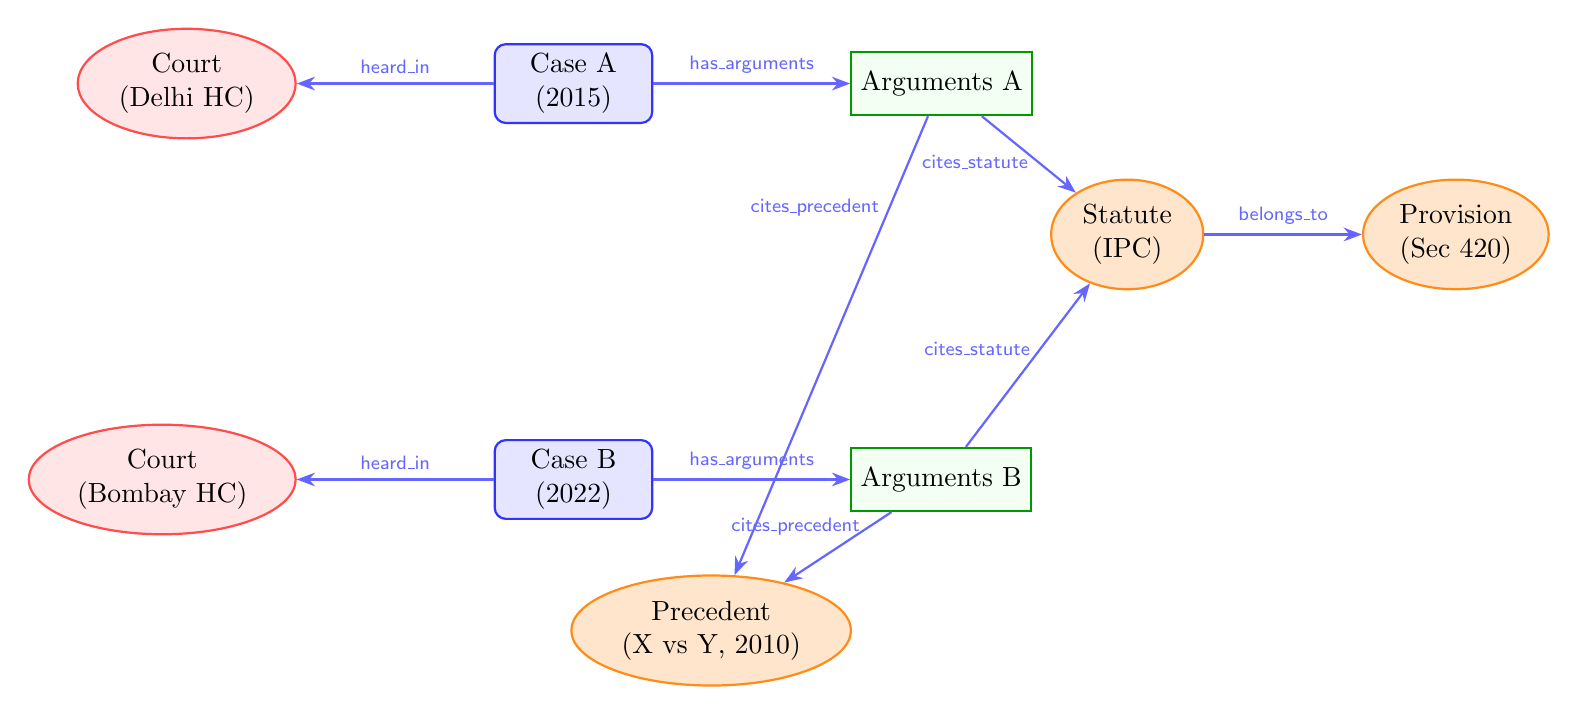
\begin{tikzpicture}[
        node distance=2cm and 2.5cm,
        case/.style={rectangle, rounded corners, draw=blue!80, fill=blue!10, thick, minimum width=2cm, minimum height=1cm, align=center},
        shared/.style={ellipse, draw=orange!90, fill=orange!20, thick, minimum height=0.8cm, align=center},
        local/.style={ellipse, draw=red!70, fill=red!10, thick, minimum height=0.8cm, align=center},
        textnode/.style={rectangle, draw=green!60!black, fill=green!5, thick, minimum height=0.8cm, align=center},
        edge/.style={->, >=Stealth, thick, blue!60, font=\scriptsize\sffamily, align=center}
    ]
        
        % Cases
        \node[case] (caseA) {Case A\\(2015)};
        \node[case, below=4cm of caseA] (caseB) {Case B\\(2022)};
        
        % Local nodes for Case A
        \node[local, left=of caseA] (courtA) {Court\\(Delhi HC)};
        \node[textnode, right=of caseA] (argsA) {Arguments A};
        \draw[edge] (caseA) -- node[above] {heard\_in} (courtA);
        \draw[edge] (caseA) -- node[above] {has\_arguments} (argsA);

        % Local nodes for Case B
        \node[local, left=of caseB] (courtB) {Court\\(Bombay HC)};
        \node[textnode, right=of caseB] (argsB) {Arguments B};
        \draw[edge] (caseB) -- node[above] {heard\_in} (courtB);
        \draw[edge] (caseB) -- node[above] {has\_arguments} (argsB);

        % Shared nodes between A and B
        \node[shared, below right=1cm and 0.5cm of argsA] (statute) {Statute\\(IPC)};
        \node[shared, right=2cm of statute] (provision) {Provision\\(Sec 420)};
        \node[shared, below left=1cm and 0.5cm of argsB] (precedent) {Precedent\\(X vs Y, 2010)};

        \draw[edge] (argsA) -- node[left, pos=0.6] {cites\_statute} (statute);
        \draw[edge] (argsB) -- node[left, pos=0.6] {cites\_statute} (statute);
        
        \draw[edge] (statute) -- node[above] {belongs\_to} (provision);

        \draw[edge] (argsA) -- node[left, pos=0.2] {cites\_precedent} (precedent);
        \draw[edge] (argsB) -- node[left, pos=0.2] {cites\_precedent} (precedent);

    \end{tikzpicture}
    \caption{\textcolor{blue}{Cross-connection of cases via shared nodes. While each case maintains its own local representations for Court, Judge, and Text Features (preventing docket-bias leakage), shared nodes like Statutes and Precedents (orange) act as cross-case conduits for message passing, allowing structural reasoning across the graph.}}
    \label{fig:cross_case_graph}
\end{figure}
}
\end{document}
